%!TEX root = ../../main.tex

\section{Evaluation}
\label{scoring:sec:eval}

Since there is no existing collection specifically for the evaluation of newsworthiness, and our overall aim is to develop a score that can be used to improve real-time event detect techniques, we evaluate our newsworthiness scoring approach on the Events 2012 corpus created and described in chapter \ref{chapter:collection}, a corpus created specifically for the evaluation of event detection approaches.

First we examine the different heuristic features defined in section \ref{scoring:sec:labelling} in the context of the Events 2012 corpus.
We then test a number of different threshold values for labelling tweets as high and low quality, and examine how Newsworthiness Scores are distributed.
We look at how different event types and categories behave, and examine how different term representations (unigrams, bigrams)  affect performance.

We process the Events 2012 corpus in a online manner, simulating a real-time stream of time-ordered tweets.
We filter out retweets and any non-English tweets. URLs are removed, and each tweet is tokenized. Unless otherwise noted, a unigram representation is used, we perform no stemming or stop word removal, and all tokens are normalized to lowercase.

\subsection{Heuristics}
In section \ref{scoring:sec:labelling}, we defined a number of heuristic features used to calculate a basic Quality Score that we then use to label tweets as either high or low quality.
We examine how these heuristics behave against tweets from the Events 2012 corpus, in terms of the percentage of tweets affected by each heuristic.
Although our heuristics are all user-based, rather than content-based, we report the number of tweets, rather than the number of unique users, as the volume of tweets affects the performance of our approach, not the number of unique users.

\subsubsection{User Description}
\begin{figure}[t!]
	\centering
	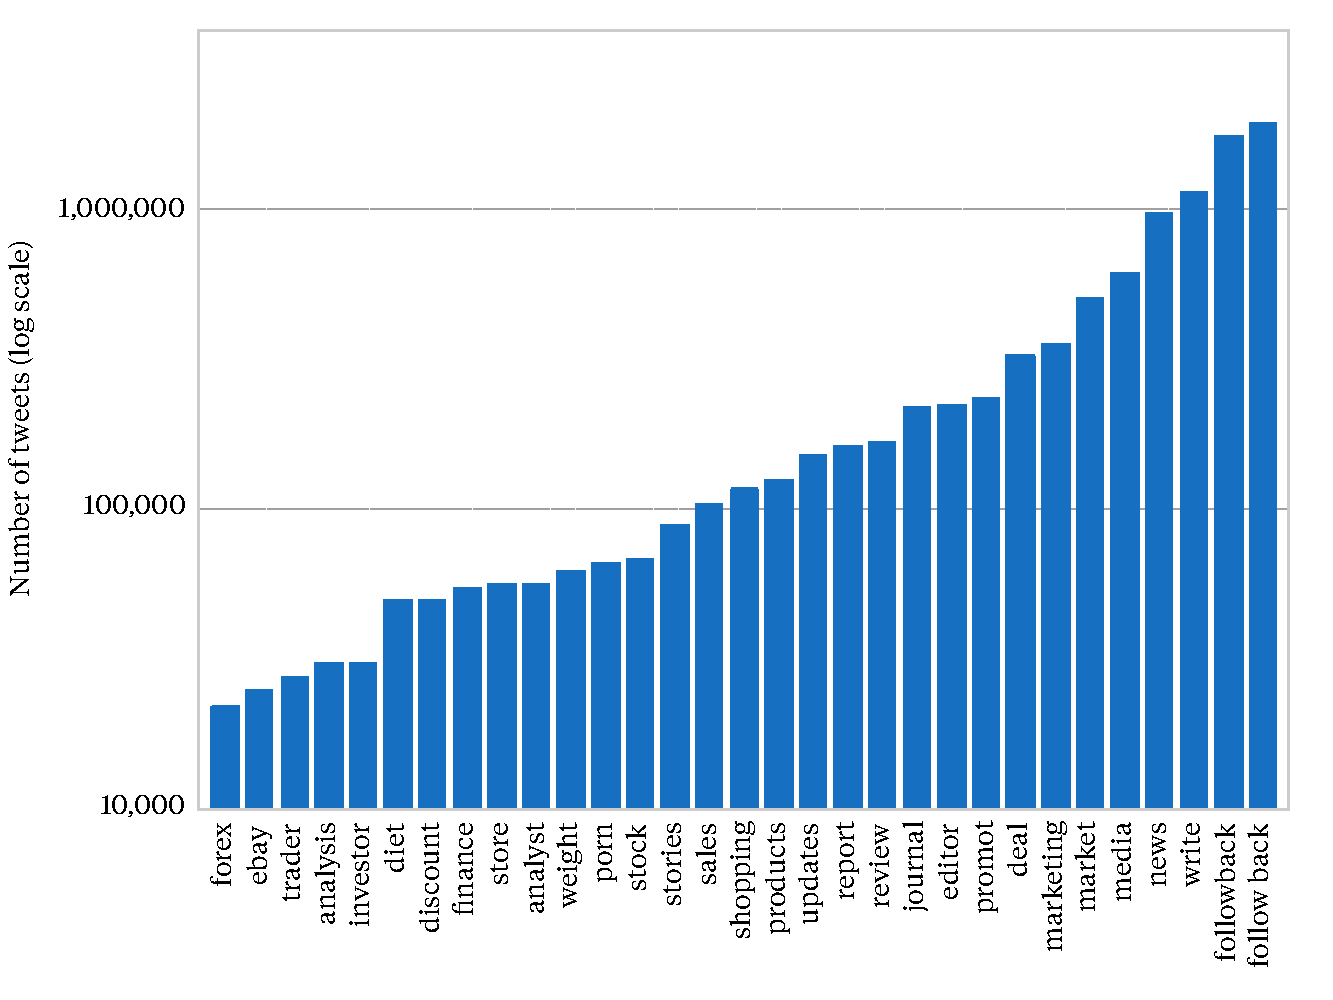
\includegraphics[width=\textwidth]{Chapters/Newsworthiness/data/descterms.pdf}
	\caption{The total number of tweets posted by users with any of the terms listed in Table \ref{scoring:table:authorKeywordsWeights}, sorted by frequency.}
	\label{scoring:graphic:descTerms}
 \end{figure}

Figure \ref{scoring:graphic:descTerms} shows the number of tweets posted by users whose User Description contains one of the terms used for scoring, sorted by raw frequency.
Note that the most common phrases  ``follow back/followback'' refer to a common type of spam described in section \ref{scoring:sec:labelling}, where a user promotes the fact that they will follow any user who follows them.
This is often used to artificially grow followers and increase the accounts perceived significance.
Since we use high numbers of followers as a positive weight, it is important that we are able to detect these accounts appropriately.

Terms relate to news and journalism appear high in the list: `media', `news' and `write' are the most common non-spam related terms, with other news and journalism related terms (`report', `journal', `editor') appearing slightly lower in terms of raw frequency.
These are extremely strong indicators that the user is either a news broadcaster or a journalist.

Finance related terms appear less frequently, with the exception of `market'. However, the bulk of this is due to the term `market' also matching `marketing', which is the next most common term.
Although `market' has a weight of 2.0, tweets by users whose description contains the phrase `marketing' (weight 0.1) will still be given an overall weight of \(2.0 \times 0.1 = 0.2\), ensuring that the overall Quality Score is kept low.
Despite the overall low frequency of financially related terms, we feel that their inclusion is important to capture discussion of financial news which may be discussed less broadly than other types of news.

\subsubsection{Followers}
Table \ref{scoring:table:followersDist} shows the number of tweets from users with particular follower ranges, and percentage of total tweets being posted by each group.
As mentioned in section \ref{scoring:sec:labelling}, the vast majority (83.81\%) of tweets are posted by users with between 50 and 4,999 followers.
This means that for the majority of tweets, this feature has no effect on the Quality Score since this range is given a weight of 1.0.
However, for tweets posted by users with fewer than 50 followers, which make up 13.78\% of tweets in the collection, this feature has a negative effect on the Quality Score. Very few tweets come from users with more than 1 million followers, a total of only 9,457 tweets, or 0.01\% of tweets in the collection, however this relatively small number of tweets will receive a significant boost in their Quality Score (\(W_{followers}\) = 3.0).

\begin{table}[h!]
	\centering
	\caption{Follower ranges and and the number of tweets posted by users (excluding retweets) within the given range of followers.}
	\begin{tabulary}{\textwidth}{l r r}
	\toprule
	\textbf{Number of Followers} & \textbf{Tweets} & \textbf{\%} \\
	\midrule
	0 - 49 & 10,358,082 & 13.78\% \\
	50 - 4,999 & 63,006,739 & 83.81\% \\
	5,000 - 9,999 & 806,565 & 1.07\% \\
	10,000 - 99,999 & 905,533 & 1.20\% \\
	100,000 - 999,999 & 90,620 & 0.12\% \\
	1,000,000+ & 9,457 & 0.01\% \\
	\bottomrule
\end{tabulary}
\label{scoring:table:followersDist}
\end{table}


\subsubsection{Posts Per Day}
Table \ref{scoring:table:postsPerDayDist} shows the number of tweets posted by users who post the specified numbers of tweets per day on average since creating their account. We can see that although the vast majority of tweets are posted by users who tweet less than 50 times per day on average, 12.4\% of tweets come from users who post more than 50 timer per day on average, meaning that these tweets will receive a Quality Score penalty under our heuristic scoring approach.

\begin{table}[h!]
	\centering

	\caption{The number of tweets in the collection (excluding retweets) from users who post various volumes of tweets per day, on average.}

	\begin{tabulary}{\textwidth}{l r r}

	\toprule
	\textbf{Average Posts Per Day} & \textbf{Tweets} & \textbf{\%} \\
	\midrule
	< 50 & 65,856,339 & 87.60\% \\
	50 - 100 & 6,334,083 & 8.43\% \\
	> 100 & 2,986,574 & 3.97\% \\
	\bottomrule
	\end{tabulary}

	\label{scoring:table:postsPerDayDist}

\end{table}

\subsubsection{Account Age}
Table \ref{scoring:table:accountAgeDist} shows the distribution of tweets posted by users with accounts of varying age.
Over 90\% of tweets are posted from accounts older than 90 days, however a not-insignificant number of posts come from accounts younger than 90 days.
A surprisingly large number of tweets, over 1\%, come from accounts created in the past 24 hours, and 9.23\% from accounts created in the past 90 days.


\begin{table}[h!]
	\centering

	\caption{The number of tweets in the collection (excluding retweets) from users who post various volumes of tweets per day, on average.}

	\begin{tabulary}{\textwidth}{l r r}

	\toprule
	\textbf{Account Age} & \textbf{Tweets} & \textbf{\%} \\
	\midrule
	< 1 day & 786,989 & 1.05\% \\
	1-29 days & 2,286,548 & 3.04\% \\
	30-90 days & 3,863,935 & 5.14\% \\
	> 90 days & 68,239,524 & 90.77\% \\
	\bottomrule
	\end{tabulary}

	\label{scoring:table:accountAgeDist}

\end{table}

\subsubsection{Verified Users}
The collection contains 110,768 tweets posted by Verified users, accounting for 0.15\% of the total tweet volume (excluding retweets).

\subsubsection{Default profile image}
The collection contains 1,574,774 tweets posted by users with the default profile image, accounting for 2.09\% of the total tweet volume (excluding retweets).


\subsection{Quality Scores}
Figure \ref{scoring:graphic:lowQualityScores} shows the percentage of tweets assigned a Quality Scores \(Q_d < 1.0\).
A total of 24,713,071 (32.87\%) tweets were given a `low' Quality Score of less than 1.0.
A large number of tweets have scores of precisely 0.5 or 0.25 (10,270,675 and 3,903,268 respectively) due to the particular weights assigned to features such as Account Age and Average Tweets Per Day.
The average low Quality Score is 0.29, with a median of 0.25.

\begin{figure}[h!]
	\centering
	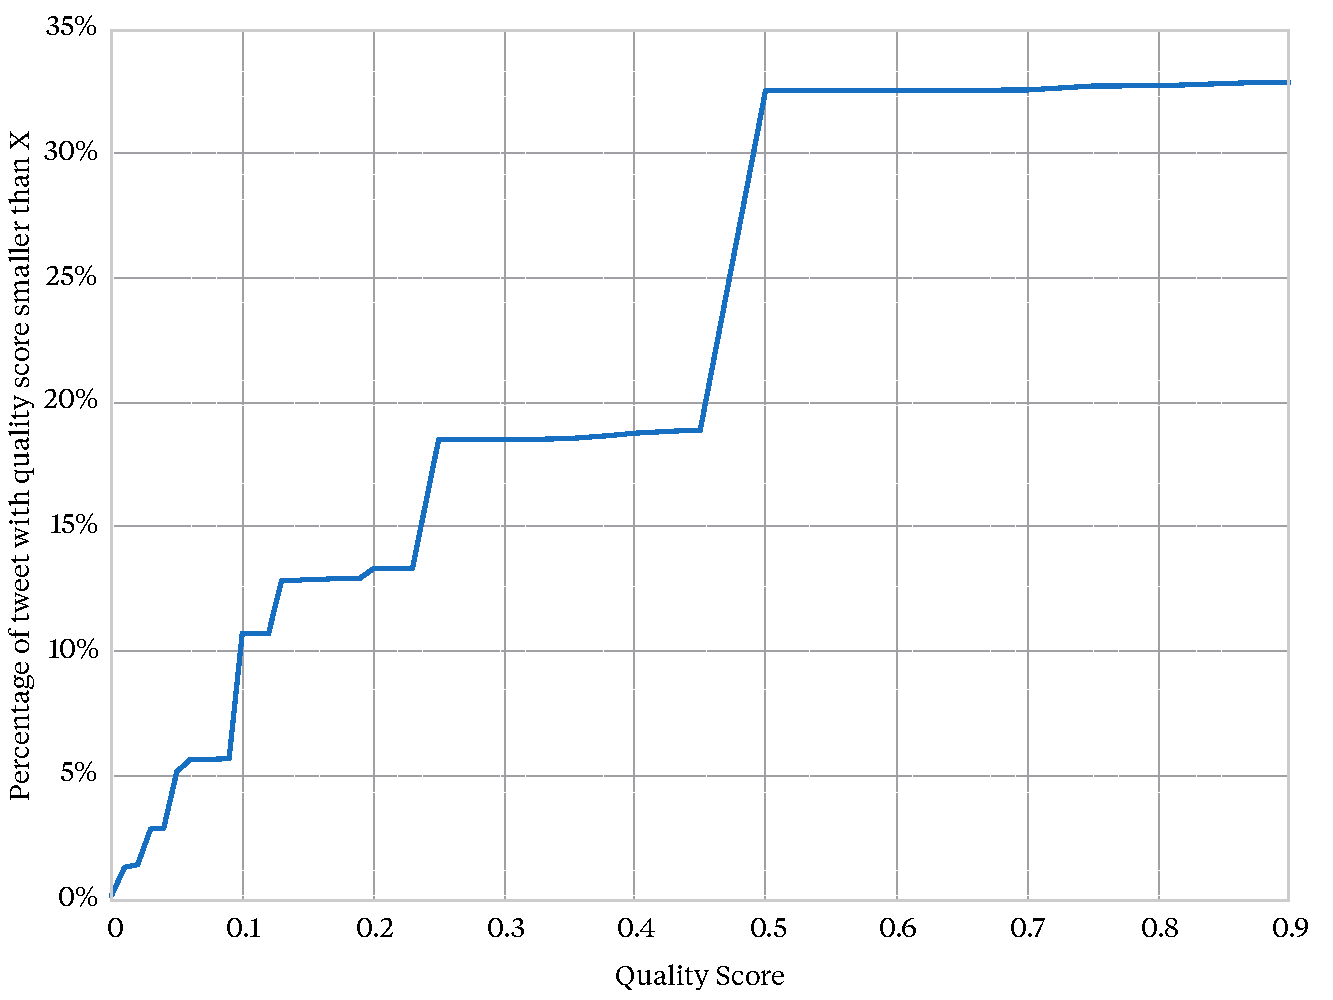
\includegraphics[width=\textwidth]{Chapters/Newsworthiness/data/negativescores.pdf}
	\caption{Cumulative percentages of tweets with Quality Score \(Q_d\) lower than the value on the x-axis, up to a maximum of 1.0}
	\label{scoring:graphic:lowQualityScores}
\end{figure}

Similarly, Figure \ref{scoring:graphic:highQualityScores} shows the percentage of tweets assigned `high' Quality Scores (i.e. \(Q_d > 1.0\)).
Note that only 3,230,830 (4.30\%) of tweets are assigned scores greater than 1.0, significantly fewer than assigned a score of less than 1.0.
The average high Quality Score is 2.46, however this is warped by a small number of outliers with extremely high Quality Scores (19 tweets have the maximum score of 224).
The median high Quality Score is 2.0.

A total of 47,233,095 (62.83\%) tweets are assigned a Quality Score of exactly 1.0, meaning that they were either assigned weights of 1.0 for all heuristic quality features, or assigned scores that cancelled.
The median score across all tweets is 1.0.


\begin{figure}[h!]
	\centering
	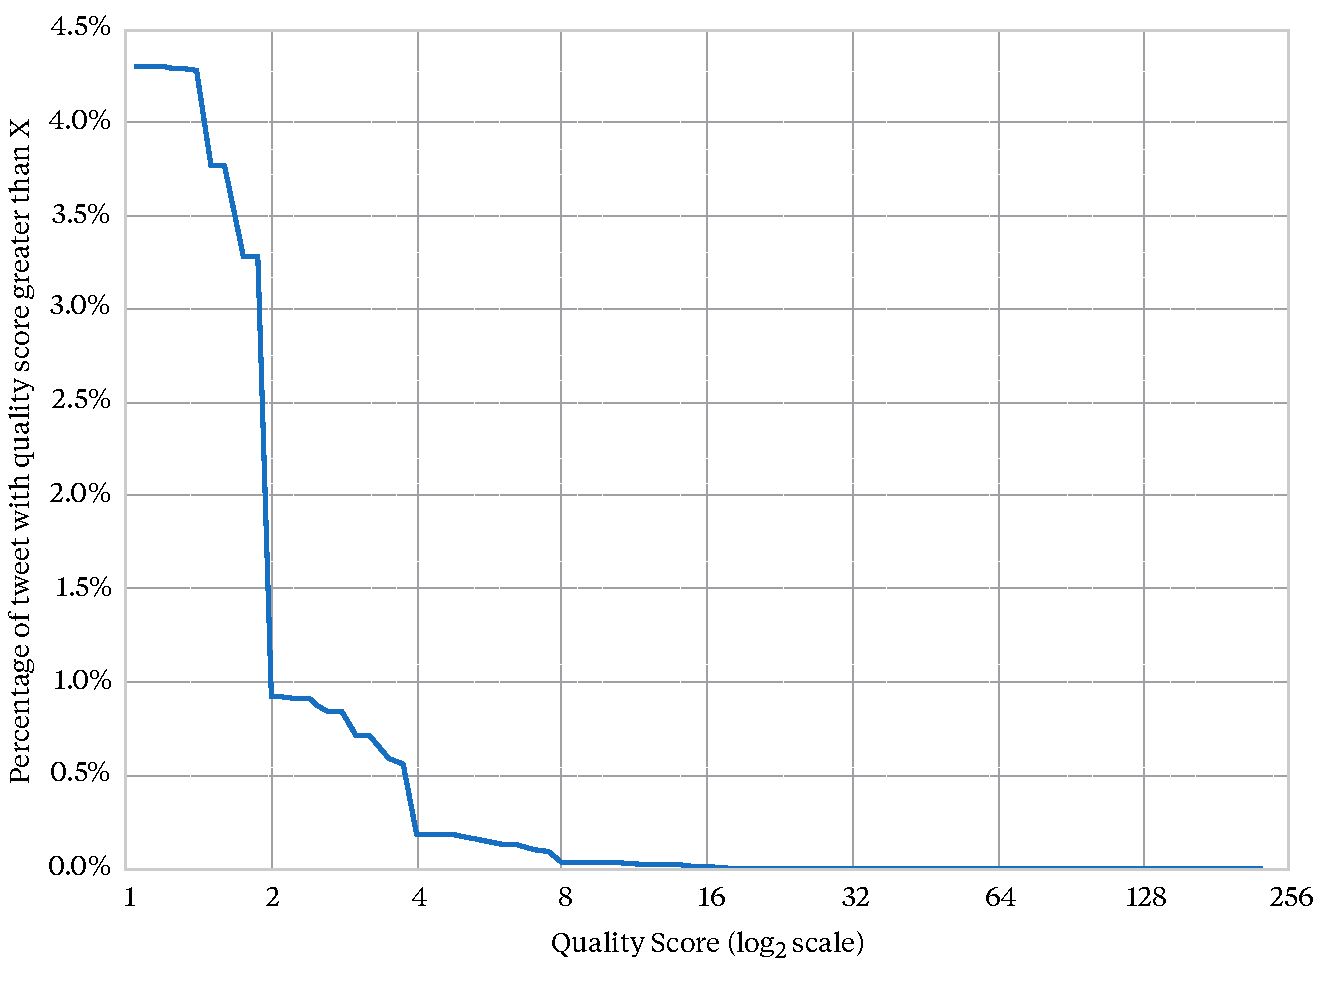
\includegraphics[width=\textwidth]{Chapters/Newsworthiness/data/positivescores.pdf}
	\caption{Cumulative percentage of tweets with Quality Scores \(Q_d\) higher than the value on the x-axis. The x-axis uses a \(log_2\) scale as the distribution is heavily skewed towards 1.}
	\label{scoring:graphic:highQualityScores}
\end{figure}

\subsection{Quality Thresholds}
We examine how different thresholds affect the overall performance of our newsworthiness predictions.
Since we lack groundtruth with appropriate Newsworthiness Scores, we instead examine the differences between scores and newsworthiness classifications for tweets known to be relevant to events in the Events 2012 corpus, and those that were not evaluated.
It is important to note that we say `not evaluated', rather than non-relevant, as  we cannot be certain that tweets that were not evaluated are not newsworthy, since only a fraction of the 120 million tweets in the Events 2012 corpus were evaluated to create relevance judgements.
It is likely that there are a significant number of unevaluated, but newsworthy tweets not included in the relevance judgements.
This means that making absolute statements is impossible.
Instead we must assume that the percentage of unevaluated but newsworthy tweets is low enough not to mask any differences in classification rates or scores.

\subsubsection{Quality Labels}

Table \ref{scoring:table:qualityLabels} shows the percentage of tweets labeled as High Quality or Low Quality. We divide tweets into two sets: those known to be relevant to an event from the Events 2012 corpus ('Event'), and all other tweets (`Other').
We also include the ratio of Event / Other tweets so that the relative percentages can be more easily compared as Quality Score thresholds are varied.
The threshold values represent the minimum or maximum scores for a tweet to be labeled as High Quality or Low Quality respectively.
For example, a tweet with a Quality Score of 2.00 would be labeled High Quality at threshold values of 2.00 and below, but not at threshold values of 4.00 or 8.00.
Similarly, a tweet with a Quality Score of 0.67 would be classified as Low Quality only if the threshold value was set to 0.67 or above.

\begin{table}[h]
	\centering

	\caption{Percentages of Event and Other tweets given High Quality and Low Quality labels at a range of Quality Score thresholds.}
	\label{scoring:table:qualityLabels}

	\begin{tabulary}{\textwidth}{c c c c}
	\toprule
	\multicolumn{4}{c}{\footnotesize \textbf{High Quality}} \\
	\textbf{Quality Score} & \textbf{Event} & \textbf{Other} & \textbf{Ratio} \\
	\midrule
	\textbf{≥ 1.25} & 12.346\% & 4.286\% & 2.881 \\
	\textbf{≥ 1.50} & 12.313\% & 4.275\% & 2.880 \\
	\textbf{≥ 2.00} & 11.505\% & 3.755\% & 3.064 \\
	\textbf{≥ 4.00} & 3.345\%  & 0.677\% & 4.944 \\
	\textbf{≥ 8.00} & 0.772\%  & 0.116\% & 6.626 \\
	\textbf{≥ 16.00} & 0.149\% & 0.017\% & 8.546 \\
	\midrule
	\multicolumn{4}{c}{\footnotesize \textbf{Low Quality}} \\
	\textbf{Quality Score} & \textbf{Event} & \textbf{Other} & \textbf{Ratio} \\
	\midrule
	\textbf{≤ 0.25} & 15.358\% & 18.497\% & 0.830 \\
	\textbf{≤ 0.50} & 31.713\% & 32.536\% & 0.975 \\
	\textbf{≤ 0.75} & 32.041\% & 32.713\% & 0.979 \\
	\bottomrule
	\end{tabulary}

\end{table}

Ratios greater than 1.0 for High Quality labels suggests that Event tweets are more likely to be labeled as High Quality than a tweet selected at random.
Conversely, a ratio of less than 1.0 for Low Quality labels means that Event tweets are less likely to be labeled as Low Quality than a tweet selected at random.

A clear difference can be seen between Event and Other tweets.
A much higher percentage of Event tweets are labeled High Quality at each threshold compared to Other tweets, with a general trend suggesting the ratio increases with threshold for High Quality labels:
as the High Quality score threshold is increased, the ratio increases from 2.881 at 1.25 to 8.546 at 16.00.
A similar, but inverse and weaker trend can be seen as the threshold is decreased for Low Quality labels.

This is a good indication that the selected heuristics are reasonable choices, and perform better than random at labeling content, as a random baseline would show ratios close to 1 for both Low and High Quality labels.

\subsection{Effect of Quality Score $Q_d$ Thresholds on Newsworthiness Classification}

Table \ref{scoring:table:newsworthinessClassifications} gives the percentage of tweets classified as Newsworthy or Noise (i.e. Newsworthiness Scores that are greater or less than 0, respectively), across a range of Quality Score ($Q_D$) threshold combinations.
At all Quality Score thresholds tested, a higher percentage of Event tweets are classified as Newsworthy and a smaller percentage are classified as Noise, compared with Other tweets.
Compared to a random baseline, which would give similar classification rates for both Event and Other tweets, our newsworthiness classification appears to perform well.
Event tweets are classified as Newsworthy at a ratio of approximately 4 to 1 when compared to Other tweets, and classified as Noise only one third as often as Other tweets.
The deviation from a ratio of 1 suggests that our Newsworthiness Scoring approach is effective at separating newsworthy content from noise.

\begin{table}[b!]
	\centering

	\caption{Percentages of tweets classified as either Newsworthy or Noise for Event and Other tweets, across a range of Quality Score threshold values.}
	\label{scoring:table:newsworthinessClassifications}

	\begin{tabulary}{\textwidth}{c c c c c c}
	\toprule
	\multicolumn{2}{c}{\footnotesize \textbf{$Q_d$ Thresholds}} & \multicolumn{2}{c}{\footnotesize \textbf{Newsworthy}} & \multicolumn{2}{c}{\footnotesize \textbf{Noise}} \\
	\textbf{HQ} & \textbf{LQ} & \textbf{Event} & \textbf{Other} & \textbf{Event} & \textbf{Other}  \\
	\midrule
	\textbf{1.25} & \textbf{0.75} & 49.759\% & 11.146\% & 6.649\% & 19.138\% \\
	\textbf{1.25} & \textbf{0.50} & 50.334\% & 11.287\% & 6.696\% & 19.218\% \\
	\textbf{1.25} & \textbf{0.25} & 61.537\% & 13.694\% & 5.736\% & 19.678\% \\
	\midrule
	\textbf{1.50} & \textbf{0.25} & 61.564\% & 13.713\% & 5.738\% & 19.682\% \\
	\textbf{2.00} & \textbf{0.25} & 64.122\% & 14.370\% & 6.601\% & 22.218\% \\
	\textbf{4.00} & \textbf{0.25} & \textbf{76.504\%} & \textbf{18.830\%} & \textbf{14.567\%} & \textbf{50.133\%} \\
	\textbf{8.00} & \textbf{0.25} & 72.748\% & 17.137\% & 18.834\% & 66.536\% \\
	\textbf{16.00} & \textbf{0.25} & 65.307\% & 17.232\% & 22.650\% & 67.193\% \\
	\bottomrule
	\end{tabulary}
\end{table}

Varying the LQ threshold appears to have only a small overall effect on the classification rates between 0.75 and 0.5.
However, once the threshold is dropped to 0.25, a more substantial change occurs.
This can likely be explained by the volume of tweets with scores below these thresholds, which remains around 32\% between 0.75 and 0.5, but drops to 18\% for 0.25, as can be seen in Table \ref{scoring:table:qualityLabels}.

The percentage of tweets classified as newsworthy reaches a maximum when we use a HQ threshold of 4.00.
Referring back to Table \ref{scoring:table:qualityLabels}, we can see that only 3.345\% of Event tweets have a Quality Score that meets or exceeds this threshold and would be used by the HQ model.
Despite this, 76.504\% of Event tweets are classified as newsworthy, but only 18.830\% of Other tweets are, giving a ratio of 4.063.
As the HQ threshold increases, the average tweet quality also increases, but decreases the volume of tweets added to the model.
This has the effect of reducing noise, and seems to benefit our newsworthiness scoring approach by increasing the proportional probability of newsworthy terms.
However, increasing the HQ threshold offers improvements only to a point, as the percentage of Event tweets given positive Newsworthiness Scores decreases as we increase the HQ threshold above 4.0.
The is likely due to the volume of tweets added to the HQ model drops sharply to less than 1\% of Event tweets above a Quality Score of 4.0, causing the model to miss important and useful information.

As overall classification ratios seem to reach a maximum around 4.0 and 0.25 for HQ and LQ thresholds, we use these thresholds for all experiments that follow.

\subsection{Newsworthiness Scores}
\begin{table}[b!]
	\centering
	\caption{Percentages of tweets classified as either Newsworthy or Noise for Event and Other tweets, across a range of Newsworthiness Score threshold values.}
	\begin{tabulary}{\textwidth}{l c c c | l c c c}
		\toprule
		\multicolumn{4}{c|}{\footnotesize \textbf{Newsworthy}} &	\multicolumn{4}{c}{\footnotesize \textbf{Noise}} \\
		\textbf{Score} & \textbf{Event} &  \textbf{Other} & \textbf{Ratio} & \textbf{Score} & \textbf{Event} &  \textbf{Other} & \textbf{Ratio} \\
		\midrule
		\textbf{> 0.0} & 76.504\% & 18.830\% & 4.063 & \textbf{< 0.0} & 14.567\% & 50.133\% & 0.291 \\
		\textbf{≥ 1.0} & 71.109\% & 16.223\% & 4.383 & \textbf{≤ -1.0} & 10.262\% & 47.076\% & 0.218 \\
		\textbf{≥ 2.0} & 59.848\% & 11.117\% & 5.383 & \textbf{≤ -2.0} & 6.964\% & 34.800\% & 0.200 \\
		\textbf{≥ 3.0} & 40.301\% & 4.701\% & 8.573 & \textbf{≤ -3.0} & 2.752\% & 16.797\% & 0.164 \\
		\textbf{≥ 4.0} & 11.707\% & 1.147\% & 10.207 & \textbf{≤ -4.0} & 0.575\% & 5.240\% & 0.110 \\
		\textbf{≥ 5.0} & 1.342\% & 0.221\% & 6.078 &\textbf{≤ -5.0} & 0.111\% & 1.562\% & 0.071 \\
		\textbf{≥ 6.0} & 0.183\% & 0.046\% & 3.969 & \textbf{≤ -6.0} & 0.024\% & 0.519\% & 0.047 \\
		\textbf{≥ 7.0} & 0.030\% & 0.011\% & 2.858 & \textbf{≤ -7.0} & 0.014\% & 0.245\% & 0.058 \\
		\bottomrule
	\end{tabulary}
	\label{scoring:table:newsworthinessScores}
\end{table}

Table \ref{scoring:table:newsworthinessScores} shows the percentage of tweets classified as Newsworthy or Noise across a range of Newsworthiness Scores.
For Newsworthy tweets, we can see that as the minimum Newsworthiness Score increases towards 4.0, the ratio of Event to Other tweets increases from 4.063 to 10.207;
whilst 11.707\% of Event tweets have a Newsworthiness Score of 4.0 or greater, only 1.147\% of Other tweets do.

Similarly, for Noise tweets, the ratio of Event to Other tweets decreases as we decrease the maximum Newsworthiness Score.
The smaller ratio in this case means that Event tweets are less likely to be classified as Noise than Other tweets.
We stop at -7.0 as no Event tweet had Newsworthiness Score of -8.0 or lower.

These results are encouraging, and follow a reasonable score distribution. The increasing and decreasing ratios for Newsworthy and Noise tweets respectively suggests that Newsworthiness Scores do incorporate some notion of newsworthiness magnitude, something we examine more closely in sections \ref{scoring:sec:categories} and \ref{scoring:sec:exampleTweets}.


\subsection{Event Categories}
\label{scoring:sec:categories}

\begin{table}[b!]
	\centering
	\caption{The raw counts and percentages per category of tweets classified as Newsworthy or Noise.}

	\small
	\begin{tabulary}{\textwidth}{l r r r}
		\toprule
		\textbf{Category} & \textbf{Newsworthy (\%)} & \textbf{Noise (\%)} & \textbf{Unclassified (\%)} \\
		\midrule
		Armed Conflicts \& Attacks 			& 8425 (97.613)  & 120 (1.390)   & 86 (0.996) \\
		Arts, Culture \& Entertainment	& 3477 (42.105)  & 2609 (31.594) & 2172 (26.302) \\
		Business \& Economy 						& 3589 (90.746)  & 127 (3.211)   & 239 (6.043) \\
		Disasters \& Accidents 					& 4196 (85.146)  & 453 (9.192)   & 279 (5.662) \\
		Law, Politics \& Scandals 			& 33197 (89.620) & 3031 (8.183)  & 814 (2.198) \\
		Miscellaneous 									& 2004 (53.698)  & 856 (22.937)  & 872 (23.365) \\
		Science \& Technology 					& 1958 (82.896)  & 133 (5.631)   & 271 (11.473) \\
		Sports 													& 19077 (62.892) & 7127 (23.496) & 4129 (13.612) \\
		\bottomrule
		\end{tabulary}
	\label{scoring:table:categories}
\end{table}

Table \ref{scoring:table:categories} shows the distribution of tweets labeled Newsworthy,  Noise, or Unclassified (i.e., Newsworthiness Scores greater than, less than, or exactly 0 respectively) across the different event categories defined by the Events 2012 corpus.
Category scores vary considerably around the mean values of 76.504\% for Newsworthy and 18.497\% for Noise (taken from Table \ref{scoring:table:newsworthinessClassifications}).
Table \ref{scoring:table:categoryScores} shows the average overall Newsworthiness Score across all Event tweets for each category, as well as independently calculated averages for tweets classified as Newsworthy or Noise.

Table \ref{scoring:table:categories} shows that over 97\% of tweets discussing Armed Conflicts and Attacks events are classified as Newsworthy, whereas only 42.105\% of Arts, Culture \& Entertainment tweets are.
This disparity can also been seen in the average Newsworthiness Scores for both categories: Armed Conflicts \& Attacks has an average Newsworthiness Score of 3.317, whilst Arts, Culture \& Entertainment has an average of only 0.427, although this difference is reduced when looking at averages for tweet classified as Newsworthy only (3.428 and 2.806, respectively).
This difference seems intuitive: armed conflicts and attacks, such as bombings, school shootings and assassination attempts are extremely newsworthy events that are likely to make headlines worldwide.
On the other hand, entertainment events, such as the launch of new television shows, or award ceremonies such as the Black Entertainment Awards, are less likely to make worldwide headlines but will still generate a high volume of subjective and low quality discussion.

Other categories behave similarly to Armed Conflicts \& Attacks, such as Business \& Economy, where events are generally headline news, but generate a relatively low volume of discussion.
Sports and Miscellaneous events, such as Felix Baumgartner's record-breaking jump from the edge of space or the start of Daylight savings time in the United States, show similar behaviour to Arts, Culture \& Entertainment.
These types of events generate a high volume of low quality chatter, resulting in a lower percentage of tweets classified as Newsworthy and lower average Newsworthiness Scores.

\begin{table}[]
	\centering

	\caption{Average Newsworthiness Scores for each event category, calculated for all tweets, only tweets classified as Newsworthy, and only tweets classified as Noise.}

	\begin{tabulary}{\textwidth}{l c c c}
		\toprule
		& \multicolumn{3}{c}{\footnotesize \textbf{Average Newsworthiness Scores}} \\
		\textbf{Category} & \textbf{All Tweets} & \textbf{Newsworthy} & \textbf{Noise}  \\
		\midrule
		Armed Conflicts \& Attacks & 3.317 & 3.428 & -2.044 \\
		Arts, Culture \& Entertainment & 0.427 & 2.806 & -2.388 \\
		Business \& Economy & 3.260 & 3.659 & -1.880 \\
		Disasters \& Accidents & 2.329 & 2.913 & -1.645 \\
		Law, Politics \& Scandals & 2.620 & 3.040 & -1.274 \\
		Miscellaneous & 0.803 & 2.249 & -1.764 \\
		Science \& Technology & 2.613 & 3.294 & -2.089 \\
		Sports & 1.044 & 2.410 & -2.007 \\
		\bottomrule
		\end{tabulary}
	\label{scoring:table:categoryScores}
\end{table}

\subsection{Example Event: Lenovo overtakes HP}
Table \ref{scoring:table:tweetsSample} gives a sample of tweets from Event \#81 of the Events 2012 corpus, sorted by Newsworthiness Score from highest to lowest.
The event describes how Lenovo, a Chinese computer manufacturer, has taken the top spot from HP in terms of number of PCs sold worldwide.
The judgements for this event identify 41 tweets thought to be relevant to the event.
Whilst the 36 of the 41 tweets are relevant, our newsworthiness scoring approach correctly identifies a number of spam and non-relevant tweets and scores them appropriately.

Two non-relevant reviews of Lenovo laptops have been given scores of 0.0 and -0.507. By themselves, these tweets are unlikely to be newsworthy, and the scores could be considered appropriate.
Our approach does give a slightly negative score to one relevant tweet (``John Cusack says Lenovo overtakes HP''), however the tweet is fairly informal in tone, and outwith the context of the other tweets would be difficult to interprate even for a human.

Note that the same text appears twice in Table \ref{scoring:table:tweetsSample}: ``HP, Lenovo battle for top spot in PC market - Computerworld''.
Although the text is identical, these are distinct tweets, posted by different users at different times, and given different scores (2.177 / 2.070).
The difference in scores is due to the adaptive nature of our newsworthiness scoring approach.
As new tweets are processed, the models are updated in real-time, allowing for new information to be incorporated and used to score subsequent tweets, resulting in the score difference.

\label{scoring:sec:exampleTweets}
\begin{table}[]

	\caption{A sample of tweets and their Newsworthiness Scores from Event \#81 of the Events 2012 corpus, sorted by Newsworthiness Score from highest to lowest.}

	\centering
	\small
	\begin{tabulary}{\textwidth}{l L}

	\toprule
	\textbf{Score} & \textbf{Tweet} \\
	\midrule
	4.102 & H-P, Lenovo jockey for No. 1 in PCs: reports: SAN FRANCISCO (MarketWatch) Hewlett-Packard and Lenovo were jockey...  \\
	3.411 & Lenovo knocks HP off top of global PC market: Gartner: SAN FRANCISCO (Reuters) - China's Lenovo Group...  \\
	2.177 & HP, Lenovo battle for top spot in PC market - Computerworld  \\
	2.070 & HP, Lenovo battle for top spot in PC market - Computerworld  \\
	1.964 & Lenovo Overtakes HP as World's Top PC Maker in Q3   \\
	1.542 & Lenovo passes HP to be top PC maker: The Chinese group has a 15.7\% share of worldwide shipments of units, compare...  \\
	0.000 & Lenovo IdeaPad Yoga 11: Hands-on with the bendy Windows RT tablet -  \\
	-0.105 & John Cusack says Lenovo overtakes HP  \\
	-0.507 & Lenovo Yoga Transforming Laptop Arrives, With Friends  \\
	-1.894 & Lady's Black Laptop Bag for 15.6 inch Lenovo G560-0679AKU Notebook + An Ekatomi Hook. | Laptop Cases 15.6  \\
	-3.263 & Lenovo IBM 0764 Series Notebook / Laptop Battery 5000mAh (Replacement): Lenovo IBM 0764 Series  Notebook / Laptop...  \\
	\bottomrule
\end{tabulary}

	\label{scoring:table:tweetsSample}

\end{table}

\subsection{Term Models}
Although unigram terms are used for all experiments, it is interesting to examine how the use of bigrams affect performance.
Table \ref{scoring:table:termModels} shows how unigrams and bigrams performed using our standard test thresholds of 4.0 and 0.25 for LQ and HQ models respectively.
Bigrams consistently underperform compared to the unigram models across all quality threshold scores tested, although the differences are often very small.

\begin{table}[h!]
	\centering
	\caption{Newsworthiness classifications for Event and Other tweets using Unigram and Bigram term models.}
	\begin{tabulary}{\textwidth}{l c c c c}
		\toprule

		& \multicolumn{2}{c}{\footnotesize \textbf{Newsworthy}} & \multicolumn{2}{c}{\footnotesize \textbf{Noise}} \\
		\textbf{Model} & \textbf{Event} & \textbf{Other} & \textbf{Event} & \textbf{Other} \\

		\midrule
		\textbf{Unigram} & 76.504\% & 18.830\% & 14.567\% & 50.133\% \\
		\textbf{Bigrams} & 74.775\% & 20.829\% & 12.715\% & 54.677\% \\

		\bottomrule
	\end{tabulary}
	\label{scoring:table:termModels}
\end{table}

Table \ref{scoring:table:topTerms} shows some of the most frequent unigrams and bigrams for both the HQ and LQ models, filtered to remove any terms with likelihood ratios of less than 2.0.
Many of the high quality bigrams refer to specific incidents or events, such as `peace prize' or the infamous ``Binders full of women'' phrase used by Mitt Romney during the second U.S. Presidential Debate of 2012.
This suggests that perhaps the bigram model is over-fitting and, rather than learning a generalizable scoring model, it is learning event-specific newsworthy phrases.
Unigrams, on the other hand, are considerably more general, and tend to be verbs associated with common newsworthy event types, such as `arrested' or `shot'.
The low quality unigrams and bigrams are semantically more similar to each other, and are often associated with games, marketing and publishing.

\begin{table}[h]
	\centering

	\caption{The most frequent unigrams and bigrams with likelihood ratios of 2.0 or greater for both the HQ and LQ models.}
	\label{scoring:table:topTerms}

	\begin{tabulary}{\textwidth}{l L}

	\toprule
	 & \textbf{Unigrams} \\
	\midrule
	\textbf{High Quality} & has, says, win, check, read, vote, set, takes, join, using, writing, breaking, wins, killed, shows, closed, leads, arrested, shot, update, expected, lead, create, add, hits  \\
	\textbf{Low Quality} & completed, earned, joined, laughed, received, signed, upgrade, collected, androidgames, led, harvesting, collect, harvested, discover, correct, submitted, increase, reviews, includes, published, mount, provides, provided, determine, marketing \\
	\midrule
	&  \textbf{Bigrams} \\
	\midrule
	\textbf{High Quality} & tribute to, peace prize, top news, us your, to lead, obama campaign, binders full, for its, courtesy of, this years, post on, south africa, in india, on october, at 35, new single, talks about, says he, 1 day, the election, this weeks, heres a, new video, presidential debate, fair and \\
	\textbf{Low Quality} & step towards, pm rageofbahamut, the tribez, a member, surveys cant, 2 months, i earned, quest in, in valor, just completed, and is, this made, doing surveys, is making, club my, far from, android androidgames, androidgames gameinsight, made me, the club, completed the, rageofbahamut rageofbahamut, more look, for more, so far \\
	\bottomrule
\end{tabulary}
\end{table}
